\documentclass[a4paper]{article}

\usepackage[T1]{fontenc}
\usepackage[utf8]{inputenc}
\usepackage[italian]{babel}
\usepackage{frontespizio}
\usepackage{graphicx}
\usepackage{listings}
\usepackage{scrextend}
\usepackage[margin=1.2in]{geometry}
\usepackage[font=small,labelfont=bf]{caption}

\begin{document}
	
% ---- FRONTESPIZIO -----
\begin{frontespizio} 
 \Preambolo{\renewcommand{\frontpretitlefont}{\fontsize{14}{12}\scshape}}
\Istituzione{Università di Pisa}
\Divisione{Scuola di Ingegneria} 
\Corso[Laurea]{Ingegneria Informatica} 
\Annoaccademico{2019--2020} 
\Titolo{Titolo} 
\Sottotitolo{Sottotitolo}
\Filigrana [height=4cm,before=0.28,after=1]{./images/stemma_unipi.png} 


\Rientro{1cm} 
\Candidato{Marco Parola} 
\Relatore{Prof.ssa Lazzerini Beatrice\\Dr. Francesco Pistolesi}
\Punteggiatura{} 
 
\end{frontespizio}

% ----- INDICE -----
	\tableofcontents
	\clearpage


% ----- INTRODUZIONE -----
	\section{Introduzione}


\begin{addmargin}[1.5cm]{0cm}
\end{addmargin}
\begin{addmargin}{1.5cm}
\textit{“ Le operazioni di trasporto o di sostegno di un carico ad opera di uno o più
lavoratori, comprese le azioni del sollevare, deporre, spingere, tirare, portare o
spostare un carico, che, per le loro caratteristiche o in conseguenza delle
condizioni ergonomiche sfavorevoli, comportano rischi di patologie da
sovraccarico biomeccanico, in particolare dorso-lombari ”.} \\ \\
\end{addmargin}
Questa è la definizione di Movimentazione Manuale dei Carichi o MMC (o, in inglese, Manual Handlng of Loads, MHL), data dall'articolo 167, decreto legislativo 81/08. \\ Queste manovre, svolte quotidianamente da operai sul posto di lavoro, rappresentano una delle cause che favoriscono l’insorgere di disturbi e patologie alla colonna vertebrale. Infatti, se consideriamo i dati provenienti dagli enti di previdenza sociale relativi al tipo e ai numeri degli infortuni sul lavoro e delle malattie professionali, questi evidenziano come, a livello mondiale, a prevalere siano malattie professionali classificabili come disturbi Muscolo-Scheletrici. \\
Si rende necessario, quindi, procedere ad una corretta valutazione del rischio da movimentazione manuale di carichi, al fine di attuare idonei interventi di prevenzione e protezione che vadano a mitigare, se non annullare, eventuali danni a carico degli operatori. Considerando poi che quasi un terzo dei lavoratori dichiara di svolgere quotidianamente questo tipo di operazione, è lecito pensare che, avere uno strumento capace di analizzare il modo in cui si effettua questo task, potrebbe permettere di comprendere il problema più a fondo e cercare una soluzione mirata.\\
L'obiettivo finale è, quindi, lo sviluppo di uno strumento, che monitori costantemente, durante la giornata lavorativa, i movimenti di un operatore e valuti il rischio a cui si espone, compiendo determinati operazioni, al fine di poter correggere gli errori compiuti duramtne l'esecuzione e trovare soluzioni ergonomiche atte a migliorare la qualità e l'ambiente lavorativo.\\ \\
Lo scopo di questa tesi è analizzare i movimenti compiuti durante il \textbf{sollevamento di un carico elevato} mediante dispositivi indossabili, che contengono al loro interno sensori, da cui raccogliere dati, per poi analizzarli in un secondo momento, al fine di capire se i dispositivi hardware, utilizzati nella prima fase di storage dei dati, sono sufficienti a distinguere una operazione eseguita in modo corretto, da una eseguita scorrettamente e che potrebbe causare lesioni. Infine realizzare uno strumento che, realtime, possa avvisare un utente, ogni qual volta compia una manovra potenzialmente dannosa.


	\clearpage

% ------ CAPITOLO I: descrizione movimento ------
	\section{Movimentazione}

	\subsection{Movimento corretto}
Al fine di evitare infortuni e minimizzare l'indice di rischio, il modo corretto, per sollevare un carico, è piegare le gambe leggermente divaricate (quanto le spalle) e, mantenendo un’inclinazione lieve e costante del busto verso il carico, il quale deve essere posizionato alla minore distanza possibile dai piedi (circa 10 cm), tornare in posizione eretta facendo forza principalmente sulle gambe. \\ L'immagine di seguito riportata illustra i passaggi da seguire per un corretto sollevamento.\\

\makebox[\linewidth]{}
\begin{center}
\begin{minipage}{0.48\linewidth}
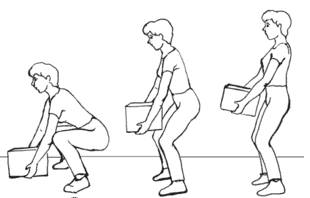
\includegraphics[width=60mm,scale=0.7]{./images/sollevamento_corretto.png} 
\makebox[\linewidth]{}
\captionof{figure}{Sollevamento corretto.}
\end{minipage}
\end{center}
\makebox[\linewidth]{}
\makebox[\linewidth]{}

\subsection{Movimento scorretto}
Un esempio di un modo scorretto di sollevare un carico è invece illustrato nella seguente figura, dove non si utilizzano le gambe, che rimangono stese durante tutta l'esecuzione della manovra, per aiutarsi nella distribuzione del peso, ma ci si piega con la sola schiena, esponendola di fatto a un alto rischio di disturbi dovuti a sovraccarico biomeccanico delle vertebre e dei dischi intervertebrali. Tale movimento è da evitare in tutti i modi. \\

\makebox[\linewidth]{}
\begin{center}
\begin{minipage}{0.48\linewidth}
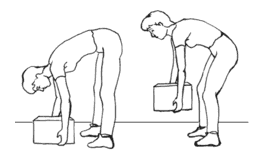
\includegraphics[width=60mm,scale=0.7]{./images/sollevamento_scorretto.png} 
\makebox[\linewidth]{}
\captionof{figure}{Sollevamento scorretto.}
\end{minipage}
\end{center}




	\clearpage

% ----- CAPITOLO II -------
	\section{Raccolta dati}
Per poter eseguire uno studio del rischio che corre una persona, sollevando un carico elevato, si affronta una prima fase in cui si raccolgono i dati relativi alla movimentazione di quest'ultima. \\
Dunque si rende necessario uno strumento che permetta di raccogliere e catalogare informazioni, con cui poter ricostruire il movimento e in una seconda fase eseguire un analisi per poter quantificare il rischio. \\



	\subsection{Sistema per la raccolta ed il salvataggio di dati}


Il sistema di cui ci muniremo dovrà contenere al suo interno sensori di vario genere, che gli permettano di registrare i movimenti e le variazioni delle condizioni ambientali esterne, a cui è sottoposto. \\
I sensori che prenderemo in considerazione, di cui l'hardware dovrà essere munito, sono i seguenti:
\begin{itemize}
\item \textbf{Accelerometro triassiale}, misura l’accelerazione che subisce il dispositivo sui tre assi cardinali.
\item \textbf{Giroscopio triassiale}, misura la velocità angolare del dispositivo attorno ai tre assi del sistema di riferimento.
\item \textbf{Magnetometro triassiale}, misura l’intensità del flusso del campo magnetico terrestre relativamente ai tre assi del sistema di riferimento. Tramite questo tipo di sensore possiamo ricavare informazioni sull’angolo che questo dispositivo forma con il campo magnetico terrestre.
\item \textbf{Barometro}, misura la pressione atmosferica alla quale il dispositivo è sottoposto; grazie alla elevata sensibilità di questo sensore è possibile individuare variazioni di pressione anche molto piccole, dell’ordine dei mbar.\\ \\
\end{itemize}

\begin{center}
\begin{minipage}{0.48\linewidth}
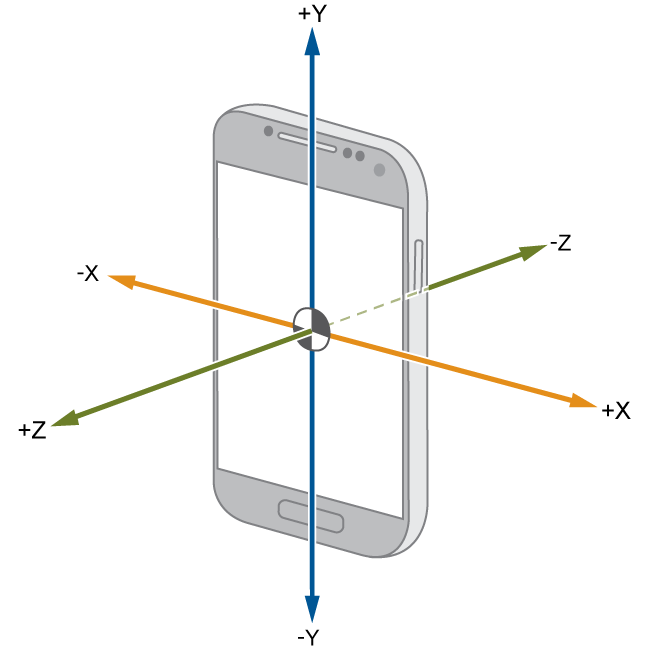
\includegraphics[width=\linewidth]{./images/triaxial_sensor.png}
\makebox[\linewidth]{}
\captionof{figure}{Sistema di coordinate (relativo allo smartphone) utilizzato dall'API Sensor.}
\end{minipage}
\end{center}


\makebox[\linewidth]{}
\makebox[\linewidth]{}
Un'altra proprietà che il nostro sistema deve possedere è essere \textbf{mini-invasivo}, infatti la persona che utilizza uno strumento di questo genere, non dovrebbe quasi accorgersi della sua presenza, affinché non si senta eccessivamente controllato oppure disturbato nei movimenti che compie; questo ci permetterà di effettuare delle misurazioni naturali e non falsate.


% ----- APPLICAZIONE ANDROID -----
	\subsection{Applicazione Android per la rccolta}
La soluzione che abbiamo trovato, che rispecchia i requisiti di sopra riportati è un'applicazione Android composta da due dispositivi hardaware: smartphone e smartwatch. \\ 
In particolare durante lo svolgimento della tesi abbiamo utilizzato uno smartphone Samsung Galaxy S6, sistema operativo Android 7.0 e uno smartwatch Huawei Watch 2, sistema operativo Wear OS 2.0 . \\
L'applicazione è stata sviluppata sull’IDE Android Studio, che integra interessanti funzionalità sia per la creazione di interfacce grafiche, sia per la parte relativa all’accesso al file system dei dispositivi compatibili.
In particolare è sviluppata in 3 moduli principali:
\begin{itemize}
\item mobile
\item wear
\item shared\_mobile\_watch \\
\end{itemize}
Il fine di questo sistema è produrre nel file system del telefono, in particolare nella directory "Documents", otto file CSV: quattro relativi allo smartphone \textit{magnetometr\_phone, gyroscope\_phone, accelerometr\_phone, pressure\_phone} e quattro relativi allo smartwatch \textit{magnetometr\_watch, gyroscope\_watch, accelerometr\_watch, pressure\_watch}; ognuno di questi 4 file descrive uno dei sensori descritti. \\


\makebox[\linewidth]{}
\begin{minipage}{\linewidth}
\begin{center}
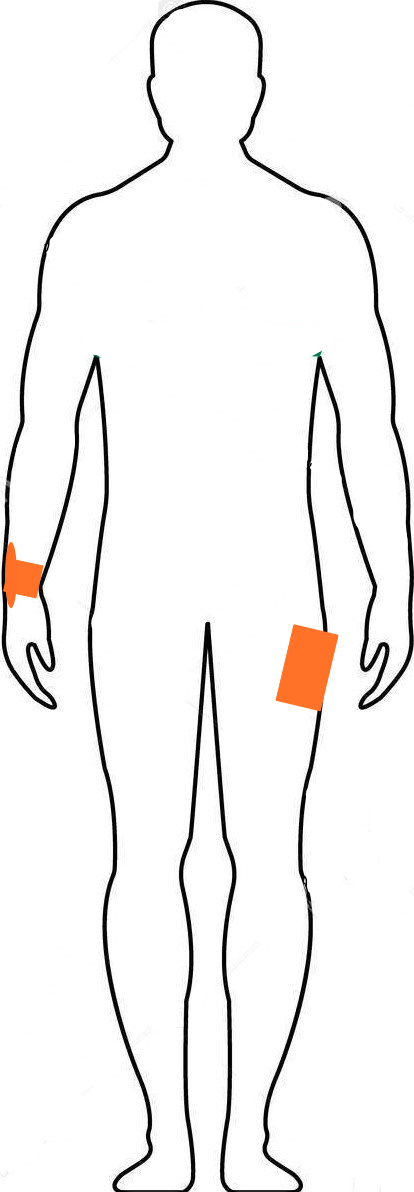
\includegraphics[width=30mm]{./images/sagoma_phone_watch.jpg} 
\makebox[\linewidth]{}
\captionof{figure}{Posizionamento dei dispositivi indossabili sull'utente.}
\end{center}
\end{minipage}
\makebox[\linewidth]{}
\makebox[\linewidth]{}


% ----- MODULO WEAR -----
\subsubsection{Modulo wear}
Il modulo wear implementa la parte dell’applicazione relativa allo smartwatch, essa ha le seguenti funzionalità: raccogliere i dati provenienti dai suoi sensori ed inviarli tramite bluetooth al telefono.\\
Di seguito non verrà riportato il codice di tutto il modulo, ma solamente la parte relativa alla raccolta dei dati e all’invio.
Nella seguente porzione di codice viene mostrato il callback che viene chiamato ogni volta che il valore di uno dei sensori subisce un cambiamento: ad ogni chiamata viene inserito nel buffer buffer (che può contenere 50 elementi) un oggetto che contiene informazioni relative al cambiamento appena avvenuto.
\makebox[\linewidth]{}
\makebox[\linewidth]{}

% ----- android wearable module -----
\begin{lstlisting}[language=Java,  basicstyle=\footnotesize]
public class MainActivity extends WearableActivity implements SensorEventListener {

    private TextView textView;
    private SensorManager sensorManager;
    ArrayList<Sensor> sensorList;
    DataSensor buffer[];
    int quanti;
    int iterazione = 0;
    ArrayList<Integer> type;
    boolean running;

    @Override
    protected void onCreate(Bundle savedInstanceState) {
        super.onCreate(savedInstanceState);
        setContentView(R.layout.activity_main);
        textView = findViewById(R.id.text);

        // register sensor
        sensorManager = (SensorManager) getSystemService(Context.SENSOR_SERVICE);
        sensorList = new ArrayList<Sensor>();
        sensorList.add(sensorManager.getDefaultSensor(Sensor.TYPE_MAGNETIC_FIELD));
        sensorList.add(sensorManager.getDefaultSensor(Sensor.TYPE_GYROSCOPE));
        sensorList.add(sensorManager.getDefaultSensor(Sensor.TYPE_ACCELEROMETER));
        sensorList.add(sensorManager.getDefaultSensor(Sensor.TYPE_PRESSURE));

        quanti = 0;
        buffer = new DataSensor[50];
        for(int i=0; i<50; i++)
            buffer[i] = new DataSensor();

        running = false;
        setAmbientEnabled();
    }

    public void startButton(View v) {
        if(!running) {
            Log.i("start", "start");
            Toast.makeText(getBaseContext(), "Start recording...", Toast.LENGTH_LONG).show();
            for (Sensor s: sensorList) {
                sensorManager.registerListener(this, s, SensorManager.SENSOR_DELAY_FASTEST);
            }
            running = true;
        }
    }

    public void stopButton(View v)
    {
        if(running) {
            Log.i("stop", "stop");
            Toast.makeText(getBaseContext(), "Stop recording...", Toast.LENGTH_LONG).show();
            sensorManager.unregisterListener(this);
            running = false;
        }
    }

    public void onSensorChanged(SensorEvent event) {

        buffer[quanti].setSensorType(event.sensor.getType());
        buffer[quanti].setTimestamp(String.valueOf(event.timestamp));
        buffer[quanti].setValue0(String.valueOf(event.values[0]));
        if(event.sensor.getType() != Sensor.TYPE_PRESSURE){
            buffer[quanti].setValue1(String.valueOf(event.values[1]));
            buffer[quanti].setValue2(String.valueOf(event.values[2]));
        }

        quanti++;

        if (quanti == 50) {
            new SendMessage("/data", buffer).start();
            for(int i=0; i<50; i++){
                Log.i("data" + iterazione + " " + i, buffer[i].getSensorType()+" ");
            }
            quanti = 0;
            iterazione++;
        }
    }

    public void onAccuracyChanged(Sensor sensor, int accuracy) {}

    class SendMessage extends Thread {
        String path;
        DataSensor message[];

        //Constructor for sending information to the Data Layer//
        SendMessage(String p, DataSensor m[]) {
            path = p;
            message = m;
        }

        public void run() {

            //Retrieve the connected devices//
            Task<List<Node>> nodeListTask =
                    Wearable.getNodeClient(getApplicationContext()).getConnectedNodes();
            try {

                //Block on a task and get the result synchronously//
                List<Node> nodes = Tasks.await(nodeListTask);
                for (Node node : nodes) {
                    try {
                        ByteArrayOutputStream bos = new ByteArrayOutputStream();
                        ObjectOutputStream oos = new ObjectOutputStream(bos);
                        oos.writeObject(message);

                        //Send the message//
                        Wearable.getMessageClient(MainActivity.this).sendMessage(node.getId(),
								 path, bos.toByteArray());
                        oos.close();
                        bos.close();
                    }
                    catch(IOException e){e.printStackTrace();}
                }
            }
            catch (ExecutionException e) {e.printStackTrace();}
            catch (InterruptedException e) {e.printStackTrace();}
        }
    }
}
\end{lstlisting}


% ----- MODULO SHARED -----
\subsubsection{Mosulo shared\_mobile\_watch}
Questo modulo molto semplice è una libreria android richiamata dai moduli mobile e wear e contenente un’unica classe DataSensor che implementa l’interfaccia Serializable, poichè le istanze di tale classe dovranno essere inviate dall’orologio al telefono. 
Tale classe memorizza le informazioni principali relative ad un cambiamento di valore di un sensore:  il tipo di sensore sensorType, tre valori value0, value1, value2 e l’istante in cui è avvenuto il cambiamento timestamp.
E’ buona pratica aggiungere in tutti i progetti, che contengono più moduli che lavorano con gli stessi tipi di classi, una libreria android, che contenga le classi necessarie ad entrambi; nonostante questo possa creare alcuni problemi durante la compilazione se ci sono aggiornamenti della versione.
\makebox[\linewidth]{}
% ----- android shared module -----
\begin{lstlisting}[language=Java,  basicstyle=\footnotesize]
public class DataSensor implements Serializable {
    private int sensorType;
    private String value0;
    private String value1;
    private String value2;
    private String timestamp;

    public int getSensorType() {
        return sensorType; }
    public void setSensorType(int sensorType) {
        this.sensorType = sensorType; }

    public String getValue0() {
        return value0; }
    public void setValue0(String value0) {
        this.value0 = value0; }

    public String getValue1() {
        return value1; }
    public void setValue1(String value1) {
        this.value1 = value1; }

    public String getValue2() {
        return value2; }
    public void setValue2(String value2) {
        this.value2 = value2; }

    public String getTimestamp() {
        return timestamp; }
    public void setTimestamp(String timestamp) {
        this.timestamp = timestamp; }

    public byte[] getBytes() {
        ByteArrayOutputStream bos = new ByteArrayOutputStream();
        ObjectOutput out = null;
        try {
            out = new ObjectOutputStream(bos);
            out.writeObject(this);
            out.flush();
            return bos.toByteArray();
        } catch (IOException e) {
            Log.e("DataSensor", e.getLocalizedMessage(), e);
        } finally {
            try {
                bos.close();
            } catch (IOException ex) {
                // ignore close exception
            }
        }
        return new byte[]{};
    }
}
\end{lstlisting}


% ----- MODULO MOBILE -----
\subsubsection{Modulo mobile}
In questo modulo vengono ricevuti i dati provenienti dall’orologio grazie al service MessageService, dichiarato nel manifesto.\\
\makebox[\linewidth]{}
% ----- android mobile module -----
\begin{lstlisting}[language=Java,  basicstyle=\footnotesize]
public class MessageService extends WearableListenerService {

    public void onMessageReceived(MessageEvent messageEvent) {

        if (messageEvent.getPath().equals("/data")) {
            final DataSensor[] message = getDataSensor(messageEvent.getData());
            Intent messageIntent = new Intent();
            messageIntent.setAction(Intent.ACTION_SEND);
            messageIntent.putExtra("message", message);
            LocalBroadcastManager.getInstance(this).sendBroadcast(messageIntent); }
    }

    public DataSensor[] getDataSensor(byte[] b) {
        ByteArrayInputStream bis = new ByteArrayInputStream(b);
        ObjectInput in = null;
        try {
            in = new ObjectInputStream(bis);
            return (DataSensor[]) in.readObject();
        }
        catch (IOException e) { Log.e("MainMobile", e.getLocalizedMessage(), e);}
        catch (ClassNotFoundException e) { Log.e("MainMobile", e.getLocalizedMessage(), e); }
        finally {
            try {
                if (in != null) {
                    in.close();
                }  } catch (IOException ex) {ex.printStackTrace();} }
        return null; }
}
\end{lstlisting}
\makebox[\linewidth]{}
Tale classe, non scrive direttamente i dati sul file, ma li invia in broadcast ad altri thread. Tali dati vengono ricevuti e scritti da un un thread Receiver, dichiarato nel metodo onCreate e richiamato all’avvio dell’applicazione. Ogni volta che viene inviato un buffer di 50 elementi dal service precedentemente descritto, viene invocato questo metodo del thread che riceve il pacchetto e ne trascrive i dati contenuti, chiamando la funzione writeFile(DataSensor buf[]), di cui non è riportato il codice, in quanto molto semplice (chiama la open su un file, scrive su di esso con il metodo write ed infine chiude il file con il metodo close). 

\makebox[\linewidth]{}
 % ----- android mobile module -----
\begin{lstlisting}[language=Java,  basicstyle=\footnotesize]
public void onReceive(Context context, Intent intent) {
        // ottengo un array di oggetti DataSensor da uno stream di byte
        DataSensor buffer[];
        buffer = (DataSensor[]) intent.getSerializableExtra("message");

        for(int i=0; i<50; i++){
            Log.i("data" + iterazione + " " + i, buffer[i].getSensorType() + " " );
        }
        iterazione++;
        writeFile(buffer);
    }
\end{lstlisting}
\makebox[\linewidth]{}
Sempre in questo modulo, inoltre, viene fatta la registrazione dei sensori contenuti nel telefono, similmente a come viene fatta nel modulo wear. Per evitare ripetizioni del codice nella documentazione, è omessa anche questa parte.

\makebox[\linewidth]{}


% ----- CAPITOLO SUGLI ESPERIMENTI -----
	\subsection{Esperimenti di registrazione}
Dopo essersi muniti di uno strumento che rispecchi i requisiti precedentemente elencati, si  affronta una fase in cui si eseguono uno o più esperimenti di registrazione: ogni esperimento è definito da un set di azioni, che dovranno essere svolte da un candidato, mentre il sistema di registrazione e salvataggio dei dati memorizza tutte le informazioni neccessarie a ricostruire la movimentazione compiuta.

% ----- ESPERIMENTO I -----
	\subsubsection{Esperimento 1}
Questo primo esperimento svolto è piuttosto semplice, vengono eseguite essenzialmente 3 azioni:
\begin {itemize}
\item camminata
\item sollevamento del carico 
\item rilascio del carico.
\end{itemize}
La ultime due azioni possono essere fatte in maniera sicura oppure dannosa per la schiena. \\
Di seguito è riportato uno schema del modulo:\\

\makebox[\linewidth]{}
\begin{minipage}{\linewidth}
\begin{center}
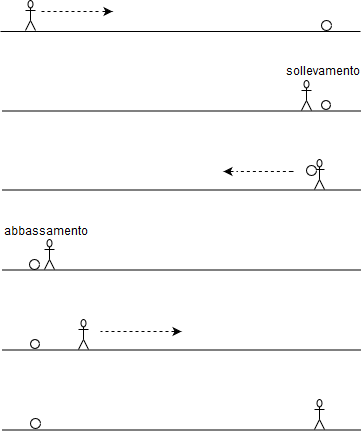
\includegraphics[width=60mm,scale=0.7]{./images/esperimento1.png} 
\makebox[\linewidth]{}
\captionof{figure}{Schema dei task dell'esperimento 1.\\}
\end{center}
\end{minipage}
\makebox[\linewidth]{} 
\makebox[\linewidth]{}
\makebox[\linewidth]{}
Questo schema riassume un ciclo del percorso totale. L’esperimento completo prevederà 2 cicli, per un totale di 2 sollevamenti e due rilasci del carico\\

\clearpage


% ------ FASE DI ANALISI ------
\section{Analisi}
La fase che segue la raccolta è l'analisi dei dati ottenuti dall'esperimento eseguito. Questo passaggio prevede l'importazione dei dati sull'ambiente di calcolo MATLAB, l'analisi e la processazione dei segnali, mediante l'utilizzo  del pacchetto Signal Processing Toolbox 8.1. \\
Questa fase di analisi si divide in due sottofasi:
\begin {itemize}
\item Individuazione dell'istante in cui avviene il task del sollevamento. L'obiettivo di questa prima fase dell'analisi è individuare gli istanti, in cui viene eseguito il movimento, in modo da non dover passare  passare alla fase della classificazione tutti i segnali dei sensori, ma solamente alcune porzioni, e rendere il sistema più efficiente.
\item Classificazione della manovra. Questa fase viene fatta da una rete neurale, che riceve in input i parametri più significativi, calcolati dalle porzioni di segnale individuate nella fase di detection, e classifica la manovra come \textit{corretta}, \textit{scorretta} o \textit{carico assente}.
\end{itemize}


% ----- ANALISI SEGNALE BAROMETRICO -----
\subsection{Il segnale barometrico per rilevare la manovra}
La prima fase di analisi ha previsto la visualizzazione dei grafici dei segnali risultanti dalle rilevazioni degli otto sensori.\\ Il sensore che dà maggiori informazioni sul momento in cui avviene l’abbassamento è il barometro dell'orologio; nel grafico, infatti, si nota che in corrispondenza di un abbassamento si ha un innalzamento della pressione atmosferica del barometro, con un conseguente abbassamento quando ci si alza nuovamente.

L’elevato livello di rumore bianco di questo segnale rende difficile il compito di trovare delle regole generali per individuare algoritmicamente il momento in cui la persona si abbassa. \\
Inoltre, il sensore è affetto da disturbi che possono influenzare l’andamento del segnale (es. correnti d’aria o le variazioni di pressione generate dall’aprire o chiudere una finestra).

\makebox[\linewidth]{}
\makebox[\linewidth]{}
\begin{minipage}{\linewidth}
\begin{center}
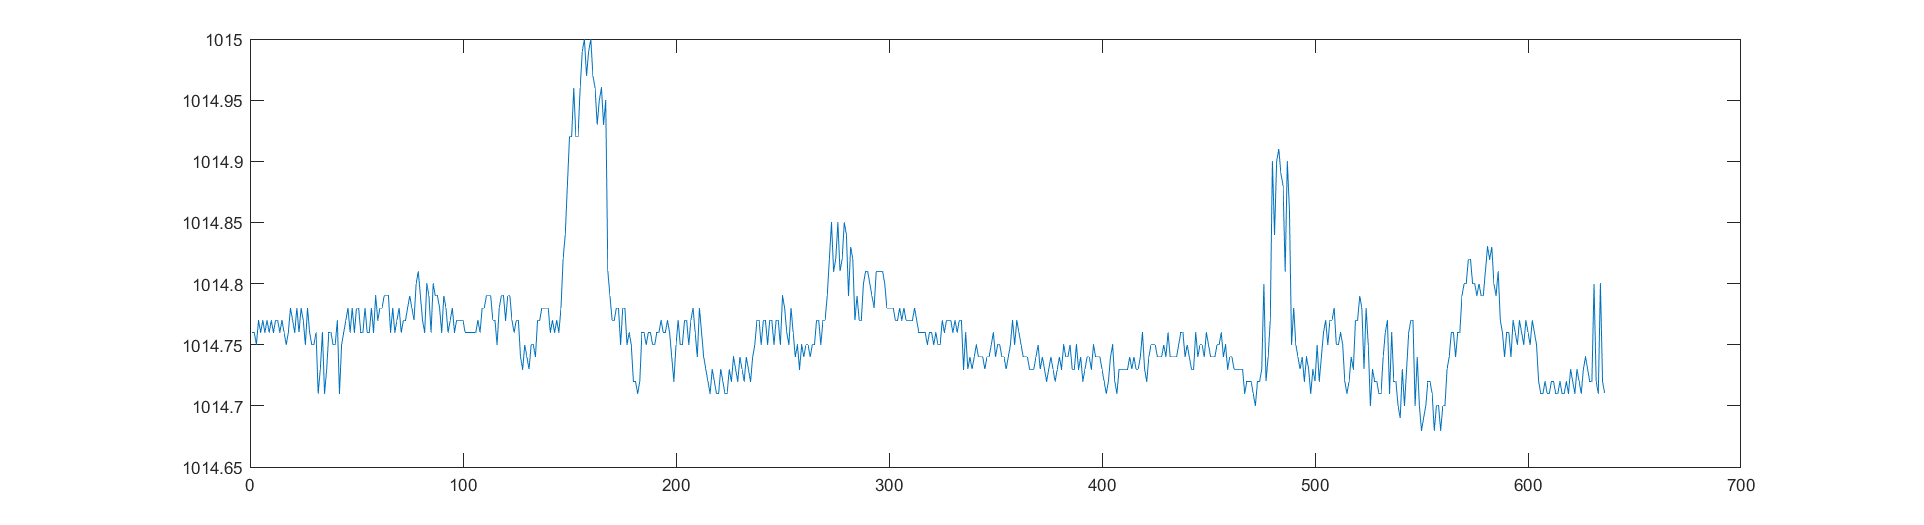
\includegraphics[width=160mm,scale=0.7]{./images/segnali/pressure_phone_grezzo.png} 
\captionof{figure}{Segnale barometrico grezzo dello smartwatch.\\}
\end{center}
\end{minipage}
\makebox[\linewidth]{}
\makebox[\linewidth]{} 
\makebox[\linewidth]{} 
%--
Per rendere più agevole la visualizzazione è opportuno applicare al segnale di partenza opportuni filtri. In particolare facendo vari tentativi, si giunge alla conclusione che, per ottenere una buonissima replica del segnale pulita e più lineare, si possono applicare un filtro a media mobile, seguito da un filtro gaussiano.
\begin {itemize}
\item Filtro a media mobile. Questo filtro prevede di ricostruire il segnale sostituendo al valore di ogni campione la media di campioni vicini. E’ una tecnica matematica utilizzata per smussare le fluttuazioni nel segnale. Si dice "mobile" perché il numero degli elementi considerati è fisso (finestra), ma l'intervallo di tempo avanza.
\item Filtro Gaussiano. Questo filtro viene applicato in cascata al precedente; anche in questo caso viene effettuata una media dei vicini, non aritmetica ma ponderata, in particolare ogni elemento verrà normalizzato, usando i coefficienti di una funzione gaussiana.
\end{itemize}
Il seguente codice Matlab applica al segnale di partenza i due filtri, producendo i grafici riportati in seguito: \\
% ----- filtri -----
\begin{lstlisting}[language=Matlab,  basicstyle=\footnotesize]
	watch_mov = movmean(pressurewatch(:,2),50);
	watchgaussian = smoothdata(watch_mov,'gaussian');
	plot(watch_mov);
	plot(watchgaussian)
\end{lstlisting}
\makebox[\linewidth]{}
\makebox[\linewidth]{}
\begin{minipage}{\linewidth}
\begin{center}
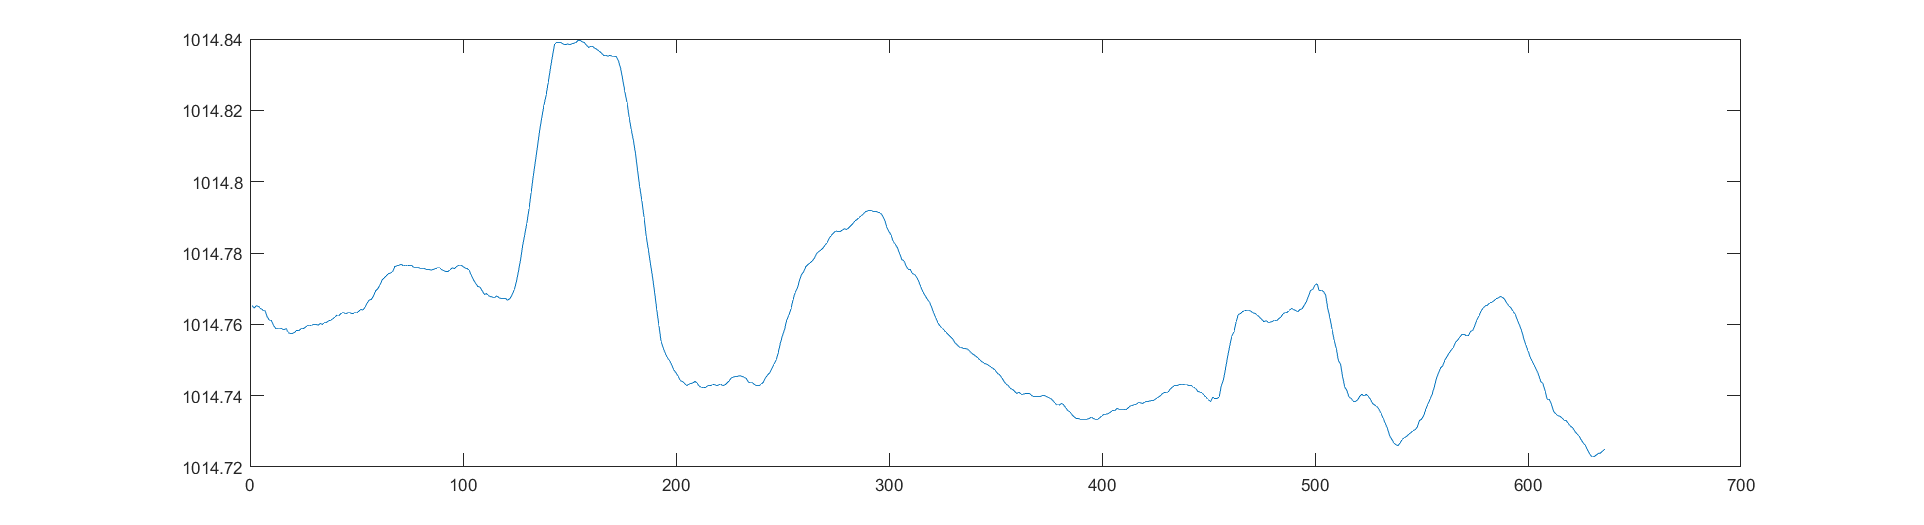
\includegraphics[width=160mm,scale=0.7]{./images/segnali/pressure_phone_movmean.png} 
\captionof{figure}{Segnale barometrico a cui è stato applicato il filtro a media mobile.\\}
\end{center}
\end{minipage}
\makebox[\linewidth]{}
\makebox[\linewidth]{}
\makebox[\linewidth]{}
\makebox[\linewidth]{}
\begin{minipage}{\linewidth}
\begin{center}
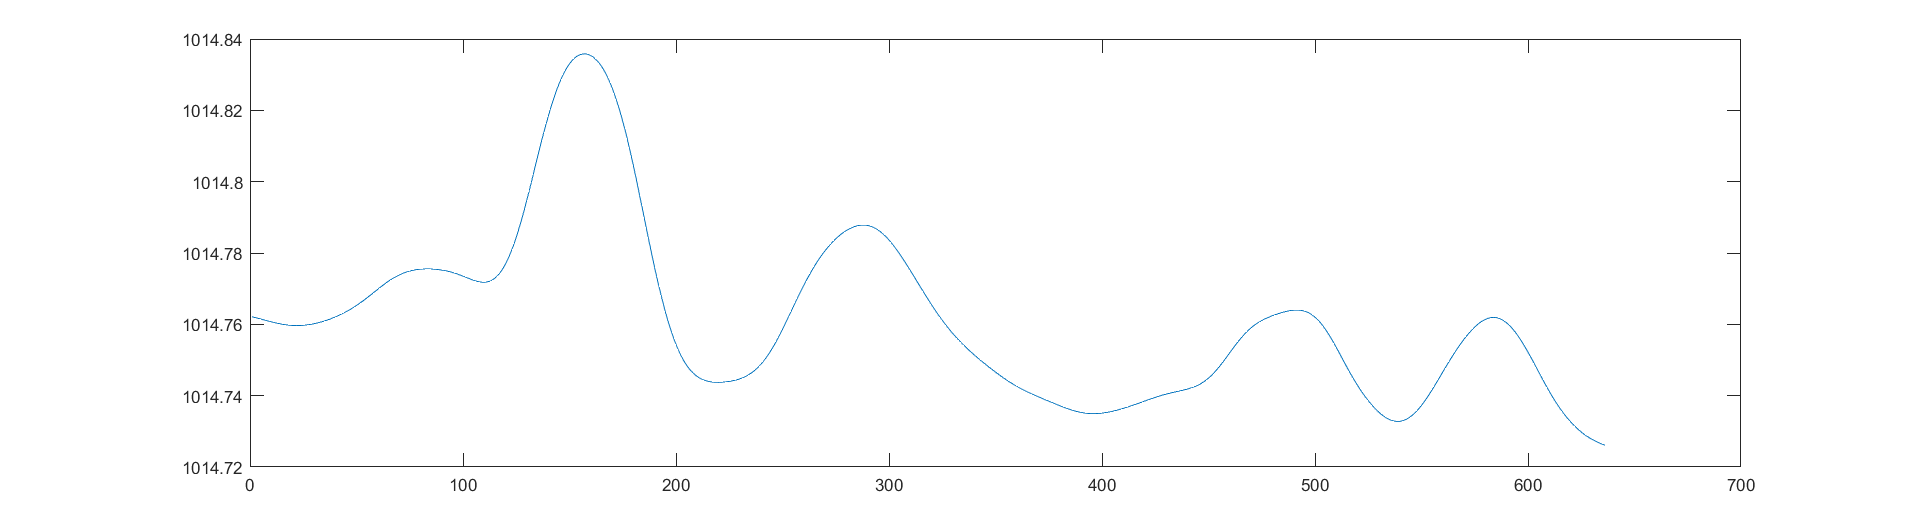
\includegraphics[width=160mm,scale=0.2]{./images/segnali/pressure_phone_gauss.png} 
\captionof{figure}{Segnale barometrico a cui sono stati applicati i filtri a media mobile e gaussiano.\\}
\end{center}
\end{minipage}


\end{document}




